Following the discovery of a scalar particle at the Large Hadron Collider (LHC), an important
question is whether this is the Standard Model (SM) Higgs boson or part of an extended Higgs
sector. One interesting approach to answer this question is to search for additional scalars,
whose observation could confirm existence of an extended Higgs sector.
For the first LHC collision data provided at a centre-of-mass energy of 13 TeV and recorded
by the ATLAS and CMS detectors, the collaborations have performed many searches that are
motivated by a variety of models beyond the SM. The simplest extensions of the SM involve the
addition of an additional singlet or doublet field, known as Electroweak Singlet Models (EWS)
and Two-Higgs-Doublet Models (2HDM), respectively. Many searches are motivated by these
extensions and benchmarks within specific related models, such as the Minimal Supersymmetric
Standard Model (MSSM). The MSSM in a particular benchmark scenario is completely
determined by two parameters, the mass of one of the Higgs bosons and the ratio of the vacuum
expectation values, tan$\beta$. In figure \ref{fig:MSSM_Run1} is shown the Run1 results by ATLAS and CMS collaborations \cite{Aad2015,CMS-PAS-HIG-16-007} .

This proceeding will detail the wide variety of new searches performed with the 13 TeV
data, which are performed with an integrated luminosity of 3.2 fb$^{-1}$ and up to 2.8 fb$^{-1}$ with the
ATLAS \cite{ATLAS-CONF-2015-061,HH_bbbb_ATLAS,HH_bbgg_ATLAS,chargedH_tb_ATLAS,chargedH_tuanu_ATLAS} 
and CMS  \cite{HH_bbtautau_CMS,HH_bbWW_CMS,HH_bbbb_CMS} detectors, respectively. Several recent results with the 8 TeV dataset were also presented \cite{Hmumu_ref_CMS,Hbb_ref_CMS,chargedH_tb_CMS,diChargedH} \cite{aa3photon}, but will not be discussed here.

 %%
\begin{figure}[htb]
\centering
	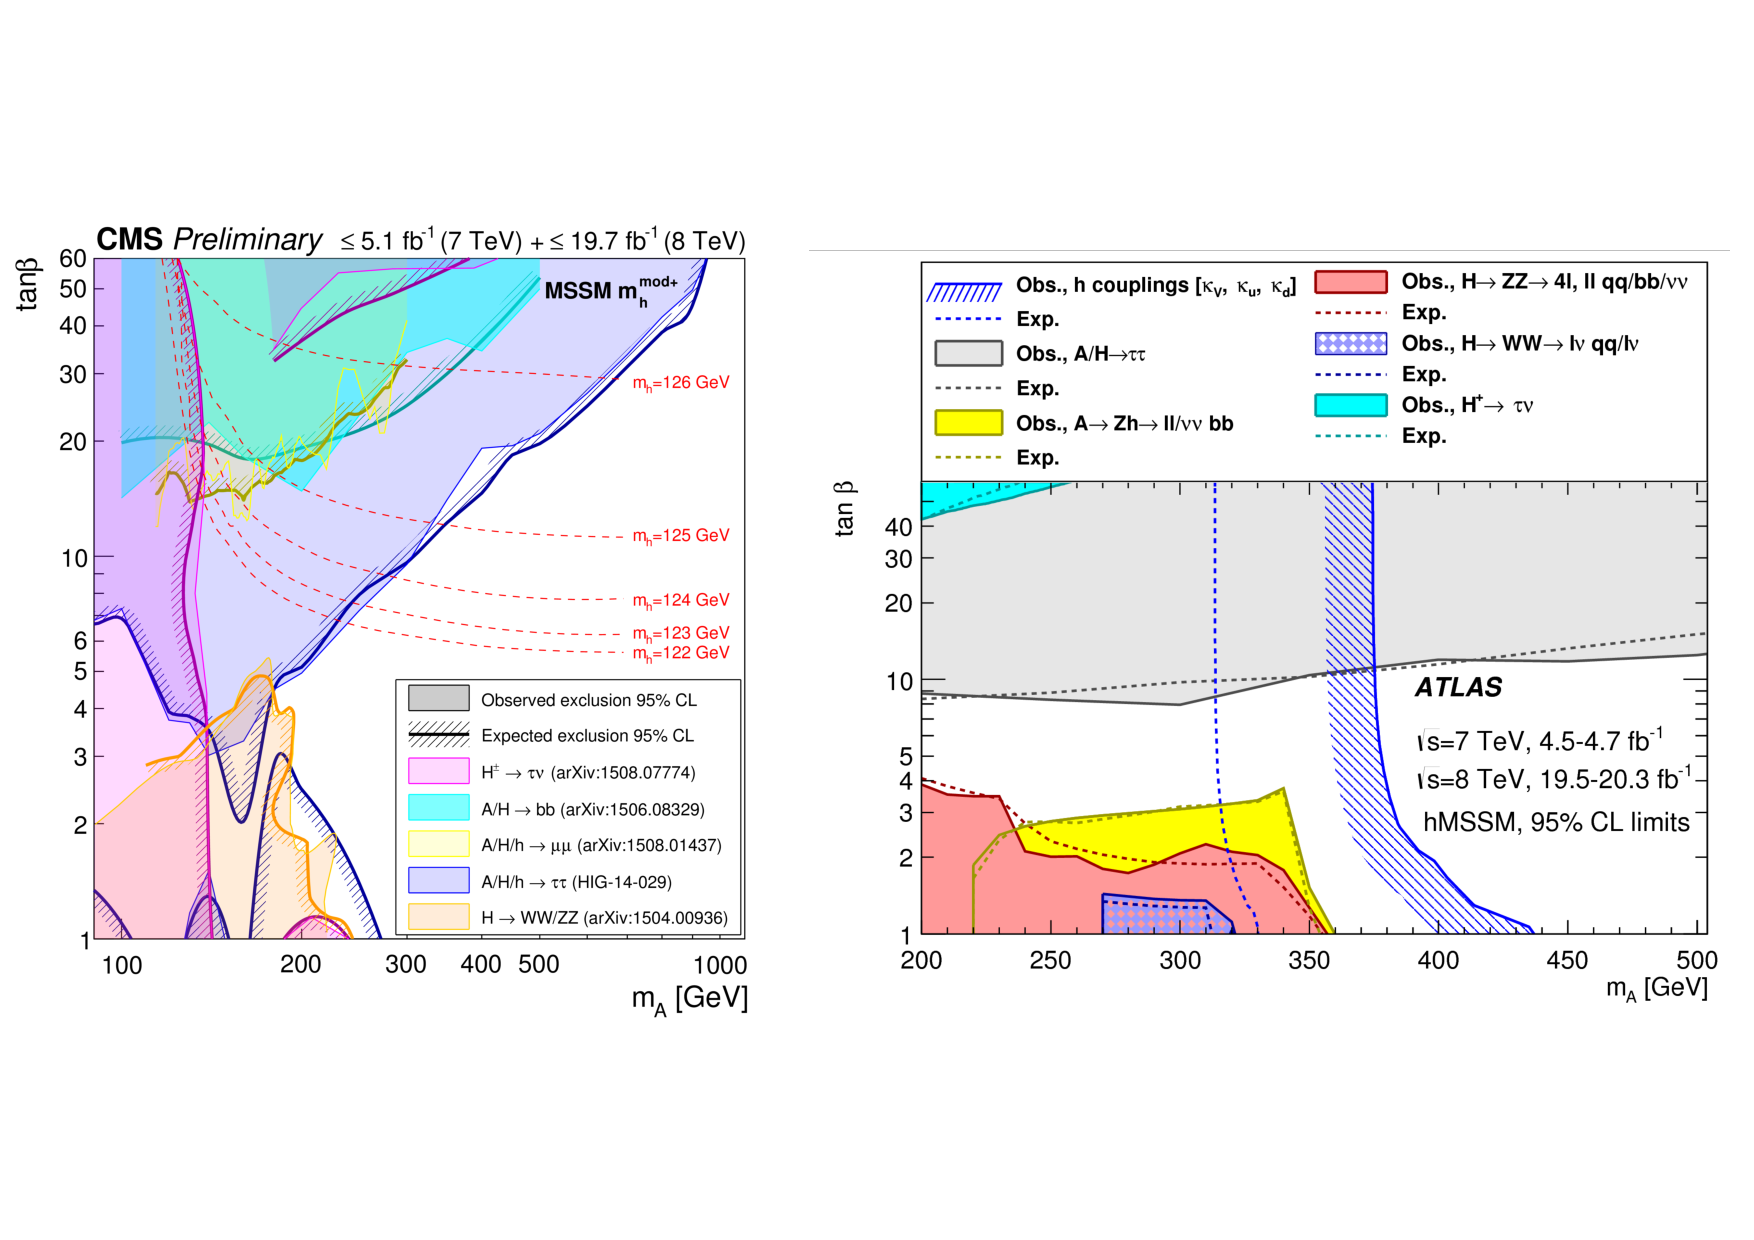
\includegraphics[width=0.9\textwidth, angle=0] {figures/MSSM_Run1.pdf}
\caption{Run1 $m_A - tan\beta$ exclusion plane by (left) CMS experiment and (right) ATLAS experiment.}
\label{fig:MSSM_Run1}   
\end{figure}
%%